% Protocol decision 2026-10-20: final-only condition-specific questionnaires; Qualtrics synchronization on hold.
\documentclass[11pt,letterpaper]{article}
\usepackage[T1]{fontenc}
\usepackage[utf8]{inputenc}
\usepackage{lmodern,microtype,amsmath,booktabs,tabularx,longtable,graphicx}
\usepackage[margin=0.8in,headheight=15pt]{geometry}
\usepackage{xcolor,fancyhdr,enumitem,xurl}
\usepackage[hidelinks]{hyperref}
\definecolor{Gold}{HTML}{987100}
\setlength{\parindent}{0pt}\setlength{\parskip}{6pt}
\setlist{nosep,leftmargin=*}\emergencystretch=3em
\pagestyle{fancy}\fancyhf{}\fancyhead[L]{\small Follow My Voice}\fancyfoot[R]{\thepage}
\newcommand{\qid}[1]{\par\smallskip\textbf{\texttt{#1}}\par}
\begin{document}
{\LARGE\bfseries Study Protocol}\par
\section{Experiment}
\subsection{Task}
Participants will perform an agent-guided object-search task while seated on a swivel chair. Multiple colored geometric objects will be scattered across eight surrounding vertical planes. The application will know the target identity, but the participant will not receive a color-and-shape description before searching. Instead, the agent will guide the participant toward the target wall and then refine the direction horizontally, vertically or diagonally. The participant will select an object using the right-controller ray and trigger. Looking at an object, receiving a gaze confirmation or pointing at it will not itself complete the trial.

Each trial will begin with the participant looking at a readiness cross. After readiness is established, an opening directional cue will play while the objects remain hidden. Object reveal will start active search timing. A correct trigger selection will stop timing and produce success feedback; an incorrect selection will be counted and search will continue. This separates readiness and opening guidance from the timed search interval while retaining their timestamps for analysis.

\subsection{Design and trial allocation}
The study will use a within-participant comparison of two voice conditions: a participant-preferred catalog voice and a self-similar synthetic voice. Both conditions will use the same guidance policy, semantic phrase library, selection method and visual-feedback settings. Actual phrase sequences may differ because guidance responds to behavior. The comparison will therefore concern voice identity within an adaptive assistance system; it will not estimate the effect of gaze contingency itself.

A saved, balanced randomized allocation will assign preferred-first or self-similar-first order. Each participant will complete two measured blocks of 40 trials, one per voice, following one practice trial. The practice trial will use the first voice in the assigned order: preferred catalog voice for Order A, or self-similar voice for Order B. Practice will be excluded from measured outcomes. A seed will make the trial and layout schedules reproducible. Nominal horizontal-angle quotas will be identical across blocks; trial order and left/right assignments will be randomized subject to those quotas.

\begin{table}[htbp]\centering
\caption{Study allocation. Nominal wall angles are schedule categories, not exact object bearings or accumulated head rotation.}
\begin{tabularx}{\linewidth}{@{}lX@{}}\toprule
Parameter & Allocation \\\midrule
Voice conditions & Preferred catalog voice; self-similar synthetic voice \\
Measured trials & 40 per block; 80 per participant \\
Practice & One trial; excluded from outcomes \\
Absolute nominal wall angle & Eight trials each at 0, 45, 90, 135 and 180 degrees per block \\
Vertical allocation & 20 targets above and 20 below readiness-cross height per block \\
Condition order & Counterbalanced preferred-first and self-similar-first \\
Selection & Right-controller ray and a trigger press \\\bottomrule
\end{tabularx}
\end{table}

Objects will vary in within-plane position, so the exact starting angle and target height will be recorded in addition to the assigned wall. The vertical allocation will use target-center height relative to the readiness cross, not the participant's seated eye height. Feasible height ranges and realized quotas will be checked in pilot schedules before the study release is frozen.

\begin{figure}[htbp]\centering
\IfFileExists{study-procedure-current.pdf}{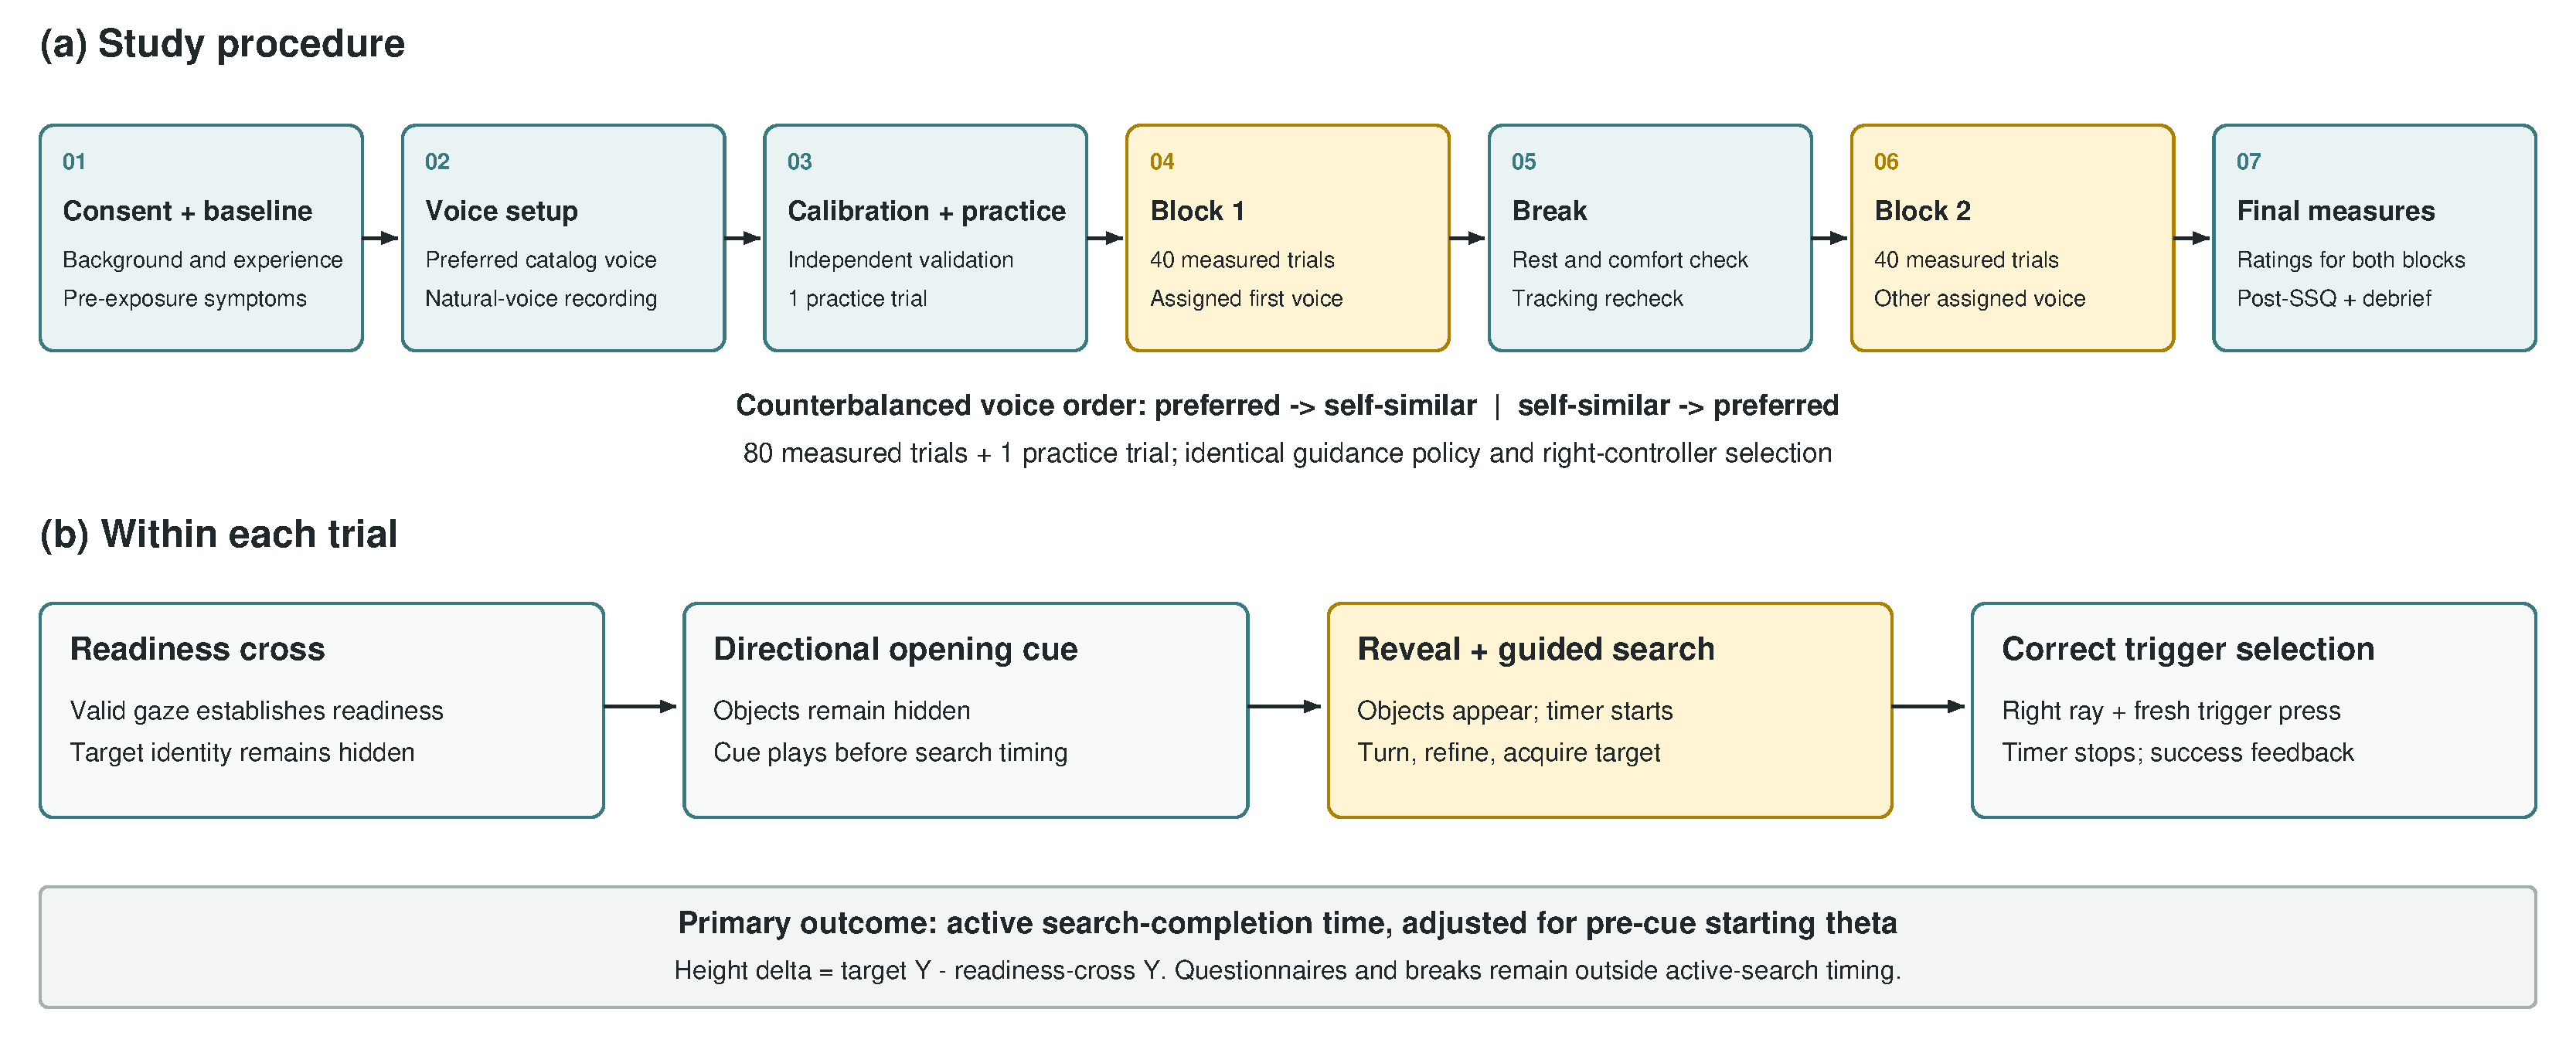
\includegraphics[width=\linewidth]{study-procedure-current.pdf}}{\fbox{\parbox{0.94\linewidth}{Consent and setup $\rightarrow$ calibration and practice $\rightarrow$ 40-trial voice block $\rightarrow$ break $\rightarrow$ 40-trial voice block $\rightarrow$ survey and debrief. Within each trial: readiness cross $\rightarrow$ opening cue $\rightarrow$ object reveal and active search $\rightarrow$ correct trigger selection.}}}
\caption{Study procedure and trial timing. Opening guidance precedes object reveal; active completion time ends at correct right-trigger selection. Questionnaires and between-trial breaks remain outside active-search timing.}
\label{fig:study-procedure}
\end{figure}

\subsection{Measures}
\subsubsection{Task performance}
\paragraph{Active completion time.} The primary outcome will be elapsed active-search time in seconds from object reveal ($t_0$) to the correct right-trigger selection ($t_1$), excluding the union of recorded pause intervals within that interval:
\[
T_{\mathrm{active}}=(t_1-t_0)-T_{\mathrm{paused}}.
\]
Lower values will indicate faster completion. Readiness, opening guidance, post-selection feedback, questionnaires and between-trial breaks will not contribute to this outcome. An unfinished trial will retain its observed exposure and outcome, but will not receive a successful completion time. The full interval from opening-cue onset to selection will be retained separately to describe the complete instructed task duration.

\paragraph{Target contact and selection errors.} Time to first target gaze will be the active-clock time of the first valid, recorded gaze-ray intersection with the target. Time to first controller contact will use the first tracked right-controller ray--target intersection. Time to final target gaze will denote the last observed valid target intersection during the trial, not a fixation duration or a spoken confirmation. These event times will remain distinct from trigger selection and from the larger gaze-vicinity region used by the guidance system. Incorrect selections will be counted as trigger selections of non-target objects. If no valid target contact is observed, its latency will remain missing rather than being set to zero. Contact times will retain their source and sampling resolution.

\subsubsection{Starting geometry and search behavior}
\paragraph{Starting angle, height and distance.} Before the opening cue, the system will record the reference origin, readiness-cross position and target position. Starting theta ($\theta_0$) will be the signed angle about world up between the horizontal origin-to-cross and origin-to-target vectors. Its magnitude $|\theta_0|$ will quantify horizontal turn demand, and its sign will preserve direction. Degenerate horizontal vectors will be marked unavailable. The primary analysis will adjust for $|\theta_0|$ rather than divide completion time by degrees. Nominal wall-angle assignment, exact pre-cue theta, and head-to-target error observed after reveal will remain separate variables.

Signed target-height difference will be $\Delta h=y_{\mathrm{target}}-y_{\mathrm{cross}}$, in metres; positive values will indicate above-cross targets. Euclidean target distance will be the three-dimensional distance between target center and the first valid tracked head position after reveal, with that observation's timestamp retained. This post-reveal distance will not substitute for a missing pre-cue geometry snapshot. All positions used in a calculation will share a recorded coordinate frame.

\paragraph{Head movement and zone coverage.} Gross head translation will sum distances between adjacent valid head positions, in metres. Gross head rotation will sum shortest quaternion angular displacements between adjacent valid orientations, in degrees. Fixed-axis component totals will be retained separately and will not be mislabeled as Euler yaw, pitch and roll. Invalid intervals, pauses and excessive sample gaps will break accumulation rather than be interpolated across; covered time and gap counts will accompany totals. These measures describe head movement, not independently tracked chair rotation.

Distinct walls visited, wall transitions and revisits will summarize search coverage using stable valid gaze observations and a versioned zone-assignment rule. Transitions across tracking gaps will not be inferred. More motion or more visits will not by themselves establish worse strategy, since geometry and available observations also affect these totals.

\paragraph{Instructions and guidance timing.} Instruction count will include guidance utterances whose playback actually starts during active search, including delivered repeats. Requested repeats, delivered repeats and interrupted utterances will be retained separately; model requests, prefetched audio and success speech will not be counted as delivered search instructions. Opening cues and success feedback will retain separate event labels. Timing analysis will distinguish evidence qualification, decision-request latency, model deferral, scheduling delay and audio onset. Gaze confirmations and controller confirmations will be evaluated separately against their corresponding evidence.

\subsubsection{Subjective measures}
\paragraph{Workload.} Six NASA-TLX dimensions---mental, physical and temporal demand, performance, effort and frustration---will be rated separately for each voice block during the final survey, after both blocks. The study will use a documented 0--10 adaptation, without pairwise weighting. Performance will run from Perfect to Failure; other dimensions will run from Very low to Very high. Individual ratings and the unweighted mean of all six completed dimensions will be retained; higher scores will indicate greater workload or poorer perceived performance. The source instrument is \href{https://doi.org/10.1016/S0166-4115(08)62386-9}{Hart and Staveland's NASA-TLX}.

\paragraph{Motivation and activity experience.} The \href{https://selfdeterminationtheory.org/intrinsic-motivation-inventory/}{Intrinsic Motivation Inventory} will contribute interest/enjoyment (7 items), effort/importance (5), pressure/tension (5), and value/usefulness (7). Responses will range from 1 = Not at all true to 7 = Very true. Published reverse keys will be applied before averaging each complete subscale. Interest/enjoyment will represent intrinsic motivation; the four subscales will not be combined into an overall IMI score. Activity wording will refer to the completed search block, with task-specific adaptations documented.

\paragraph{Agent perception.} Twenty-one items from \href{https://doi.org/10.1145/3651288}{Guo et al. (2024), Appendix A, Table A1} will assess co-presence (Q1--6), perceived intelligence (Q13--18), appealing/eerie/familiar impressions (Q20--22), and perceived anthropomorphism (Q37--42). ``Virtual character'' will be adapted to ``voice agent.'' Responses will range from 1 = Very strongly disagree to 7 = Very strongly agree. The three six-item constructs will have separate complete-scale means. Q20--22 will be analyzed individually, without a combined eeriness score. These attributed qualities will not be interpreted as actual agent intelligence or sentience.

\paragraph{Voice experience and reliance.} Twelve custom 1--7 agreement items will assess voice similarity, responsiveness, helpfulness, distraction, familiarity, trust, comfort, uncanniness, reliance, naturalness, willingness to follow and motivation to act without guidance. Voice similarity will serve as a manipulation check. Voice liking and retrospective percentage of guidance use will each use 0--100 responses with separate unable-to-answer options. These 14 numeric items will be analyzed separately; they are not a validated composite scale. Liking during voice audition will remain separate from condition-specific liking collected at the end.

\paragraph{Symptoms and debrief.} The 16 \href{https://doi.org/10.1207/s15327108ijap0303_3}{Simulator Sickness Questionnaire} symptoms will be rated from 0 = None to 3 = Severe before headset exposure and after headset removal. Canonical total or subscale scores will require the published membership and weights. Open debrief questions will explore perceived performance, guidance experience, own-voice comfort, possible use cases and voice preference; broad experience questions will precede specific eeriness or inner-dialogue probes.

Each condition-specific set in the final survey will therefore contain 65 numeric responses (130 across both sets): six workload ratings, 24 IMI items, 21 Guo items and 14 custom ratings. Technical checks and optional text will be additional. Questionnaire observations will have participant-by-block scope even when copied into per-trial summary files; they will not be treated as 40 independent responses. Missing answers will not be replaced with zero.

\subsubsection{Measurement quality}
Tracking validity, observation age, data coverage, gaps and spatial-validation error will accompany gaze-derived measures. Ray intersections and vicinity hits will not be labeled fixations, and render-frame observations will not establish native eye-tracker sampling frequency. Pupil-based workload inference and fixation/saccade outcomes will require independent validation before inclusion. Trial performance and subjective summaries will remain linked to separate raw gaze, motion and event records through participant, session, block and trial identifiers. Scale metadata will distinguish the present 0--10 workload form from any earlier exports using another range.

\subsection{Research questions}
The primary question will be whether self-similar and preferred catalog voices differ in active completion time after accounting for absolute starting theta. Secondary questions will concern workload and the four IMI subscales. Exploratory questions will concern agent perception, eeriness, voice experience, reliance, search behavior and variation in the voice contrast with starting angle. The primary voice contrast will be two-sided; a directional benefit of self-similarity will not be assumed. Repeated trials will not be treated as independent participants.

\subsection{Participants}
Participants will be consenting adults able to understand the task, hear the guidance, view the scene with usual correction and safely use the seated setup and right controller. Handedness, visual correction and prior XR and voice-assistant experience will be recorded. Recruitment size and the enrollment ceiling will be determined before recruitment using power analysis for the theta-adjusted repeated-measures outcome, including plausible within-participant variation and incomplete observations.

\subsection{Procedure}
After consent, participants will complete background questions and baseline symptom ratings. They will choose a preferred catalog voice, rate auditioned voices, record a standard passage in their natural voice for synthesis, and confirm comfortable, clear audio for each condition. Preferred gender presentation will be chosen explicitly rather than inferred from participant gender.

The researcher will fit the headset and conduct vendor calibration followed by independent spatial validation across relevant heights, wall boundaries, distances and head orientations. Validation targets will be separate from any targets used to fit an offset correction. Standardized instructions will explain that participants will rely on the agent to discover the target and use the right trigger to select it. Participants will then complete the single practice trial and the two assigned 40-trial blocks.

No questionnaire will interrupt the block sequence. During the final survey, the same condition-specific questionnaire will be completed twice, once referring to Block 1 and once to Block 2, with identical item wording and order. Breaks will be offered between trials and at the block boundary; any necessary in-trial pause will be logged immediately. Tracking will be rechecked between blocks and after headset adjustment. After headset removal, participants will first complete the final symptom check, then the two retrospective condition-specific sets, comparative voice preference and debrief. Participants may request a pause or stop, and symptoms or technical problems will prompt researcher assessment.

\subsection{Pilot testing and parameter checks}
Before confirmatory recruitment, pilot sessions will verify the realized angle/height schedules, target visibility and seated comfort, readiness and selection behavior, gaze validity, audio timing and wording, and reconstruction of trial events from the saved data. Survey comprehension and completion time will also be measured. Calibration acceptance, practice proficiency, timeout and technical-stop criteria will be set from those checks and recorded with the study build and questionnaire versions. Pilot observations will be reported as such rather than presented as study outcomes or evidence for a voice-condition effect.

\section{Guidance system}
Follow My Voice is a gaze-contingent voice guidance system that helps a seated user find a target object in a surrounding search scene. The system divides responsibility between a local guidance layer, which owns all spatial reasoning, and a cloud language model agent, Jev, which decides how and when to speak. Figure~\ref{fig:architecture} summarizes the pipeline from sensing to speech output. This division keeps task-critical decisions deterministic and auditable while allowing the agent to adapt the phrasing and timing of guidance to the user's recent behavior.

\subsection{Apparatus}
The application is developed in Unity 6 (6000.3.10f1) using the Unity OpenXR Plugin (1.16.1), HTC VIVE OpenXR integration (2.5.1), and Unity XR Interaction Toolkit (3.3.1). It is deployed as a standalone Android ARM64 application on the HTC VIVE Focus Vision head-mounted display, with rendering performed locally on the headset using the Universal Render Pipeline (17.3.0). The headset supplies head-pose and eye-gaze tracking, while the tracked right-hand controller supplies pointing and trigger input. Video passthrough supports the mixed-reality view. Network access supports cloud-based agent decisions and voice preparation; it is not used to stream rendered frames from a host computer.

\subsection{Search Task}
The search task takes place in augmented reality using video passthrough in a neutral physical room. Participants sit on a swivel chair and interact using the right controller. Virtual colored geometric objects hang on eight vertical planes anchored along the surrounding walls. Figure~\ref{fig:scene} shows the layout from above. The application holds the target identity, which is withheld from the opening instructions, so participants must rely on voice guidance to locate it. Participants select an object by pointing the controller ray at it and pressing the trigger. Stimulus density and spatial bounds will be frozen for the study release after seated-comfort and ray-selection pilots. For each trial, the system logs object positions, layout seed, wall assignment, and target identity.

\begin{figure}[htbp]\centering
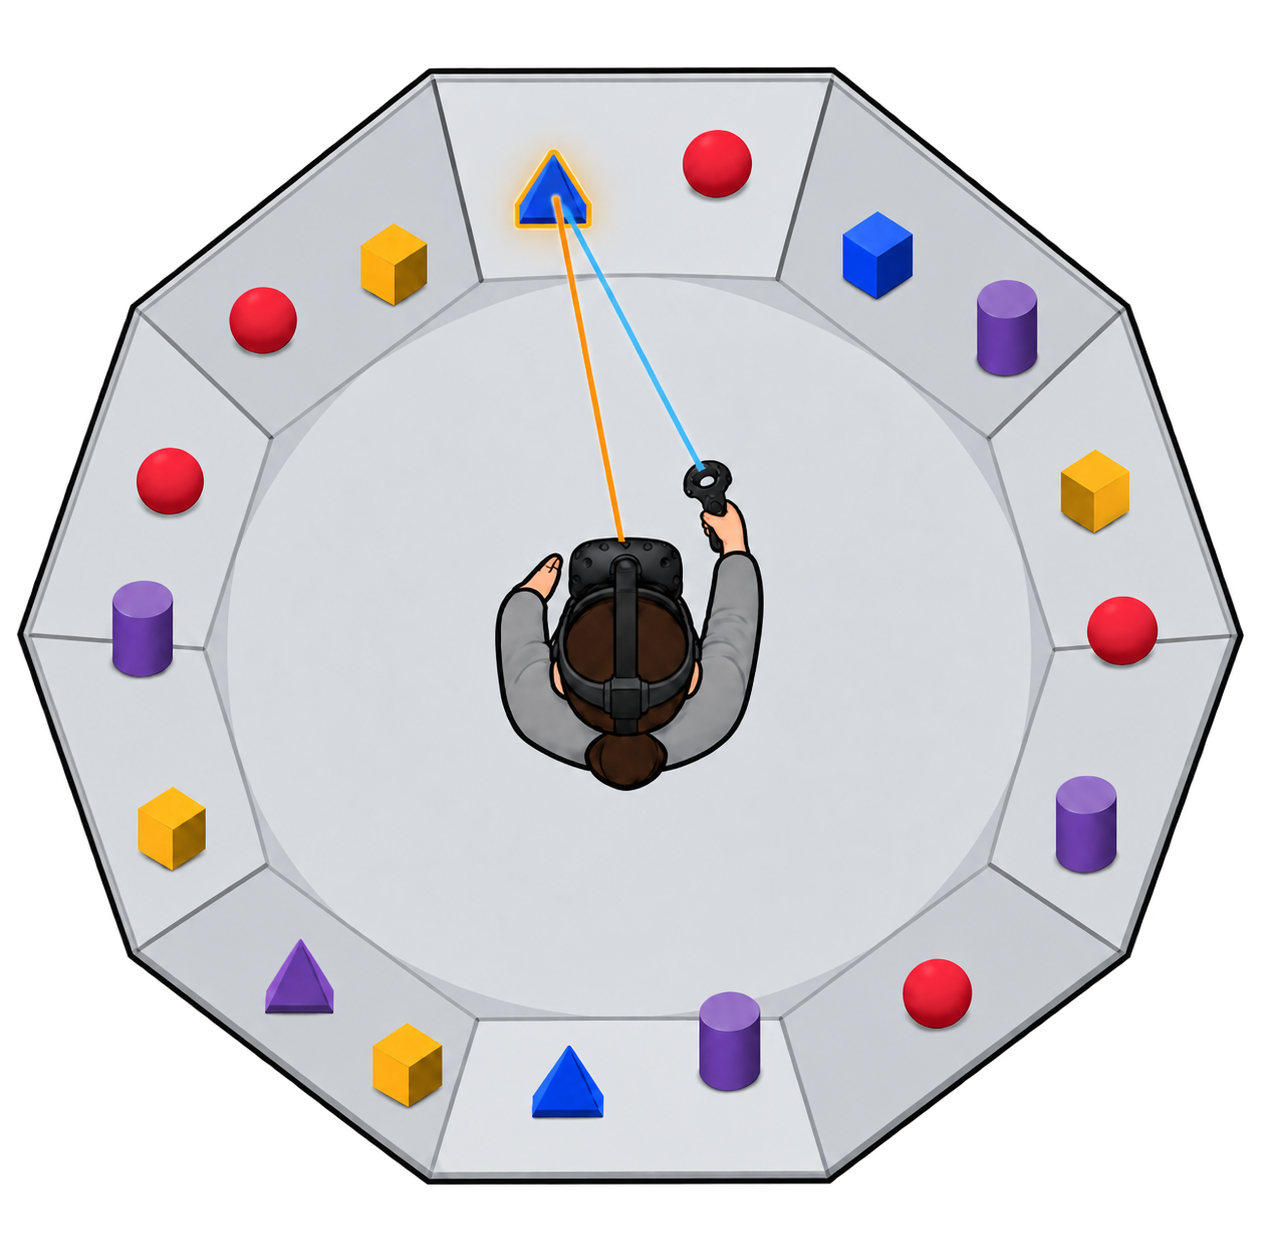
\includegraphics[width=0.6\linewidth]{image.png}
\caption{Top-down view of the search scene. The seated participant is surrounded by wall panels holding colored geometric objects. The gaze ray (orange) and controller ray (blue) converge on the highlighted target, the state in which the participant is ready to select with the trigger. The layout is illustrative; the drawn object count is schematic; object positions and target identity vary by trial.}
\label{fig:scene}
\end{figure}

\subsection{Sensing and Guidance State}
The system continuously collects eye-gaze origin, direction, and validity; head pose; right-controller pose; and ray-object intersections. A local state machine combines these observations with the target geometry to track the participant's progress through the search: turning toward the target wall, refining within the wall, acquiring the target with gaze, pointing with the controller, and becoming ready to select. Additional states cover suspended or paused operation. Each state transition is logged with its cause.

Because guidance is only as reliable as the evidence behind it, the state machine issues new gaze-dependent guidance only when gaze data are valid and recent. Gaze ray hits, gaze-vicinity candidates, and controller hits are treated as separate observations. When gaze-vicinity regions overlap, the closest object is selected. A controller hit immediately suppresses contradictory directional cues, even before the dwell required for spoken pointing confirmation has elapsed, so the system does not direct the participant away from an object they are already pointing at. Gaze confirmation, controller confirmation, and trigger selection are recorded as distinct events.

\subsection{Short-Term Interaction Memory}
To give guidance continuity, the system maintains two short-term memories. A spatial history tracks turning progress and supports cues that return the participant to the target. A speech-decision memory records what the system actually said and how the guidance state changed. Each speech entry stores its relative age, context, and whether playback completed or was interrupted; each state entry stores the prior and current states and the reason for the transition. The speech and transition lists each retain at most four entries; snapshots sent to Jev exclude entries older than 15 seconds. This bounded recent context is related to the context-management motivation of EmBARDiment~\cite{bovo2025embardiment}, but the current implementation does not use its object-admission or dropout policy. The separate spatial history retains up to three seconds or 384 target-relative gaze observations and clears on invalid evidence, source changes, or observation gaps longer than 100~ms. These limits are engineering settings, not validated fixation or blink thresholds. Gaze-vicinity confirmation currently requires 100~ms of valid qualifying evidence; invalid evidence resets its entry timer, and reacquisition after a spoken confirmation requires 150~ms of valid gaze away. Those interaction gates do not admit objects to speech memory, and missing gaze is not counted as observed dwell. The memory is cleared whenever guidance resets and is copied before each asynchronous request. This memory is deliberately scoped to the current task: it does not build a persistent participant profile or attempt to infer unobserved mental states.

\subsection{Agent Decisions and Playback Control}
Jev selects from a constrained set of options rather than generating free-form instructions. Local geometry and state rules first filter the phrase library to candidates that are valid in the current situation. Each request to Jev contains a state snapshot, recent memory, playback status, and two to five eligible phrases. Jev then chooses the wording and whether to speak now or wait. Target definition and geometric reasoning remain local. Eligibility filtering and playback revalidation reduce spatially incorrect or stale guidance, but tracking error, imperfect geometry and software faults can still produce unhelpful instructions; recorded-sequence and headset checks remain necessary.

Because cloud responses arrive asynchronously, the participant's state may change before a decision returns. A local speech scheduler therefore revalidates each decision against the current state, evidence, pacing, and object intersections before playback, and discards decisions that are stale or conflict with the current situation. Feedback that qualifies for local handling is played from prepared phrases without waiting for a new cloud decision, subject to the same checks. Each completed or interrupted utterance updates both the memory and the event log. Model latency, deferral, cancellation, fallback, and playback onset are logged separately, so any delay in speech can be attributed to the stage that caused it.

\begin{figure}[htbp]\centering
\IfFileExists{voice-guidance-memory-architecture.pdf}{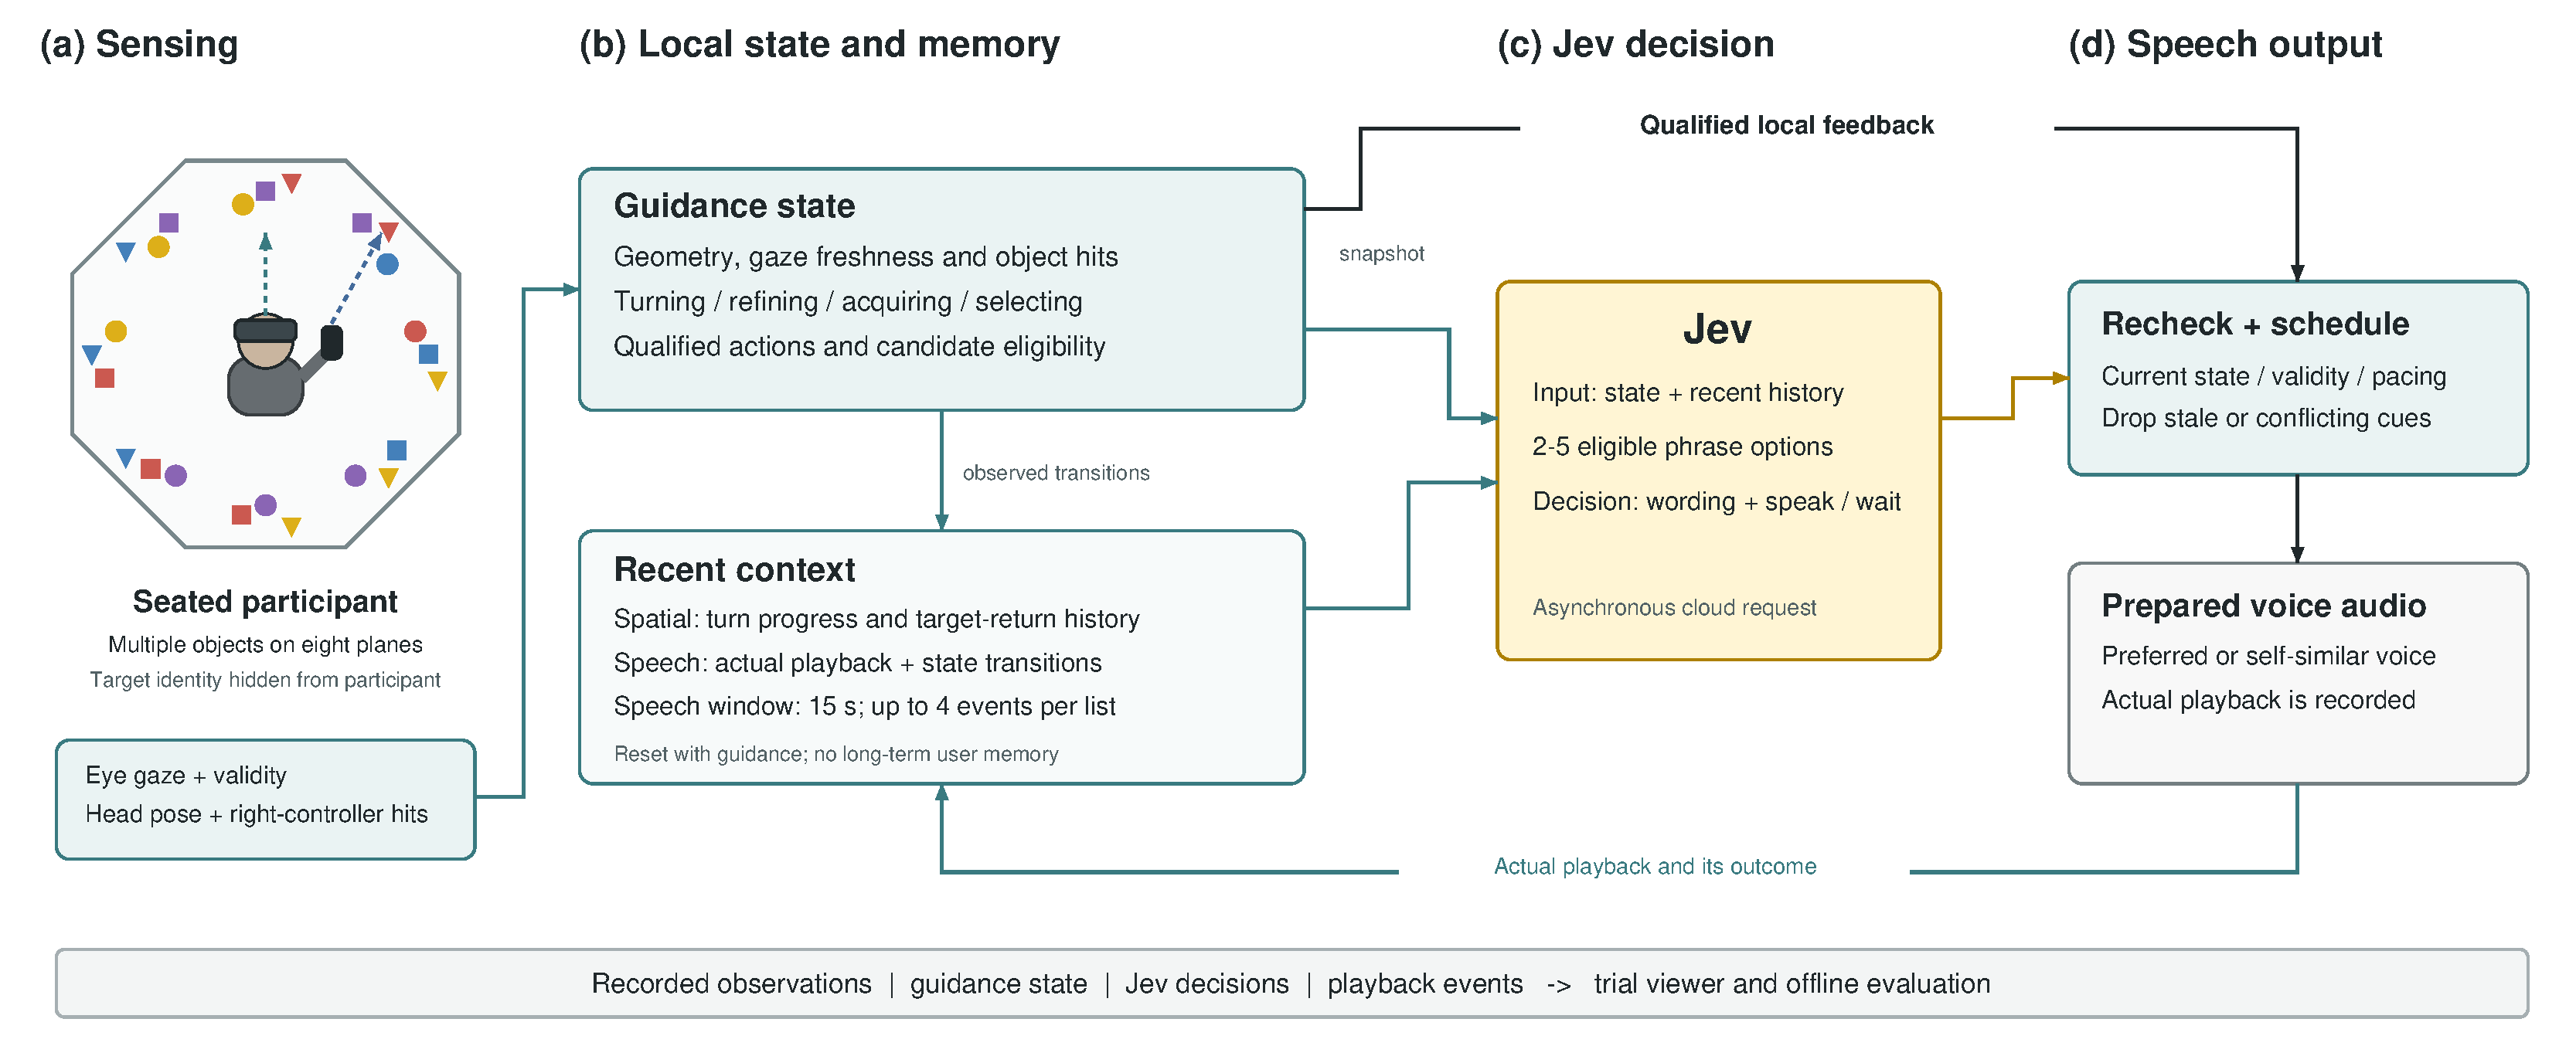
\includegraphics[width=\linewidth]{voice-guidance-memory-architecture.pdf}}{\fbox{\parbox{0.94\linewidth}{Gaze and controller observations $\rightarrow$ local state and bounded context $\rightarrow$ eligible choices for Jev $\rightarrow$ current-state recheck $\rightarrow$ prepared voice playback. Qualified local feedback also enters the recheck stage.}}}
\caption{System architecture. (a) Gaze, head, and controller data are sensed. (b) A local state machine and short-term memory determine which guidance actions are valid. (c) Jev chooses wording and timing from eligible options. (d) The scheduler revalidates each cue against the current state before playback. Actual playback feeds back into memory. The scene inset is schematic and does not reflect stimulus count or any participant-visible target cue.}
\label{fig:architecture}
\end{figure}

\subsection{Voice Preparation and Telemetry}
All voice audio is pre-synthesized with ElevenLabs, which supplies both the catalog voice and the self-similar voice. To support the self-similar condition, each participant records the same standard passage in their usual speaking voice. Both conditions share the semantic phrase library, guidance policy, and playback routing. Voice condition is the intended manipulation; behavior-dependent wording, hint counts and synthesized acoustics need not be identical. The preparation pipeline checks wording and library readiness. Per-voice intelligibility, loudness and acoustic comparability still require pilot verification; automated checks do not establish perceptual equivalence. No pitch or spatial effects are applied to the self-similar voice. We log the provider, model, voice ID, library version, and synthesis settings.

A trial viewer aligns gaze and controller state, guidance transitions, agent decisions, and playback events with trial geometry on a common timeline. Trial-level aggregates are stored separately from the raw gaze, motion, and event streams. Effective gaze sampling rate must be verified from distinct source timestamps on the tested headset build rather than inferred from the nominal specification or application polling rate. Similarly, we report ray intersections as gaze hits and do not label them as fixations unless a validated event classifier is applied.
\section{Analysis}
\subsection{Primary contrast}
The primary estimand will compare active completion time under the self-similar and participant-preferred catalog voices, standardized to the same starting-difficulty distribution. A trial-level mixed-effects analysis of log completion time will account for participant clustering, voice condition, period/order, trial progression and absolute pre-cue starting theta. Report the voice time ratio and uncertainty using a two-sided contrast.

A prespecified low-complexity function of theta will allow nonlinearity; nominal-angle strata will support balance plots and a categorical sensitivity analysis. Zero-degree trials will remain in the analysis, and completion time will not be divided by angle. The model's random-effects structure, angle function and smallest meaningful effect will be finalized with simulation before confirmatory recruitment. Participant count will be justified under that same model; repeated trials will not be treated as independent participants.

\subsection{Secondary and exploratory outcomes}
Individual workload dimensions and complete unweighted workload means will be summarized by participant and block. IMI subscales and the three six-item agent-perception constructs will remain separate scores. The additional Guo Q20--22 appealing, eerie and familiar ratings will be analyzed individually, without a combined eeriness score. Voice similarity will be a manipulation check. Custom experience ratings and self-reported guidance use will be analyzed individually. Multiplicity families and secondary contrasts will be specified before confirmatory analysis.

Instruction count, observed gaze path and other behavior potentially caused by voice condition will not automatically be covariates in the primary model. Voice-by-theta variation, selected catalog voice, acoustic quality and guidance timing will be exploratory or sensitivity analyses with their assumptions reported.

\subsection{Incomplete and interrupted observations}
Raw attempts, incorrect selections, pause intervals, timeouts, technical failures and withdrawals will be retained. Stopped trials will not be coded as successful completion times. Timeout/censoring rules and the missing-data estimand will be specified before collection; slow trials will not be removed solely for being slow. Missing responses will not be replaced with zero. Questionnaire scores will follow the complete-subscale rule, with item-level missingness reported. Disliking or failing to recognize a cloned voice will not by itself exclude a participant.

\subsection{Guidance and qualitative evaluation}
Engineering analysis will distinguish event qualification, decision latency, model deferral, scheduling delay and actual playback. Gaze and controller confirmation will be evaluated separately. Sequence-level review will include what happened before and after a cue. Automatic checks and model-judge ratings will remain advisory engineering evidence, not participant perception scores.

Debrief responses will be coded with a documented thematic process and an audit trail, with independent review of a subset. Perceived performance, voice comfort, reliance and possible own-voice use cases will be interpreted alongside, but not substituted for, measured task performance.
\section{Measures and scoring}
\subsection{Battery and timing}
After both 40-trial voice blocks, participants will complete the final survey with two separately labelled retrospective sets, one referring to each voice block. Each set will contain six workload ratings, 24 Intrinsic Motivation Inventory (IMI) items, 21 agent-perception items and 14 study-specific numeric ratings. This yields 65 numeric responses per referenced block (130 across both sets), plus technical checks and optional text, all administered at the end. Baseline and final Simulator Sickness Questionnaire (SSQ) administrations contribute 16 symptoms each. Voice setup adds a liking rating for every auditioned voice, including the self-similar voice.

\subsection{Workload}
The six NASA-TLX dimensions will be measured in the final survey once for each referenced voice block with discrete 0--10 ratings. Demand, effort and frustration will range from Very low to Very high. Performance will range from Perfect to Failure, so higher values consistently indicate worse workload/performance experience. Individual dimensions and an unweighted mean will be retained. The mean will be computed only when all six ratings are present. No pairwise weighting will be used. This 0--10 response format is a local adaptation of NASA-TLX; it will be reported as such rather than treated as an unchanged original form.
\href{https://doi.org/10.1016/S0166-4115(08)62386-9}{Hart and Staveland (1988), Development of NASA-TLX}.

\subsection{Motivation and activity experience}
Four IMI subscales will be administered in the final survey separately for each referenced block: interest/enjoyment (7 items), effort/importance (5), pressure/tension (5), and value/usefulness (7). Responses will range from 1 = Not at all true to 7 = Very true, with 4 = Somewhat true. Interest/enjoyment is the direct measure of intrinsic motivation; the other subscales describe distinct experiences.

Within-subscale item positions will be reverse-scored with $8-r$: interest/enjoyment 3 and 4; effort/importance 2 and 5; pressure/tension 1 and 3; value/usefulness none. Each complete subscale will be averaged separately. No overall IMI score will be calculated. Incomplete subscale scores will remain missing, with raw responses and the number answered retained.

``Activity'' will refer to the completed search block. Value/usefulness fill-ins will refer to practicing visual search and search performance. Pressure item 5 will read ``I felt pressured while doing this activity.'' These task-specific adaptations will be documented; reverse-key annotations will not be shown to participants.
\href{https://selfdeterminationtheory.org/intrinsic-motivation-inventory/}{Official IMI guidance and instrument materials}.

\subsection{Agent perception}
The battery will use the co-presence (Q1--6), perceived intelligence (Q13--18), the three items in the source's ``Eerie'' group (Q20--22), and perceived anthropomorphism (Q37--42) items reproduced by \href{https://doi.org/10.1145/3651288}{Guo et al. (2024), Collaborating with my Doppelg\"anger}, Appendix A, Table A1. \href{https://web.ics.purdue.edu/~cmousas/papers/jour24-PACMCGIT-SelfSimiarAppearanceVoice.pdf}{Author-hosted full text}.

Guo attributes co-presence to Biocca, Harms and Gregg (2001), perceived intelligence and anthropomorphism to Moussawi and Koufaris (2019), and the ``Eerie'' group to Zibrek et al. (2018). The source evaluates an embodied virtual collaborator. The present questionnaire will replace ``virtual character'' with ``voice agent'' and use it/its/itself pronouns. This transfer does not establish validation for a disembodied voice agent.

Responses will range from 1 = Very strongly disagree to 7 = Very strongly agree. Source IDs will be preserved in exports as GUO2024\_Q1--Q6, Q13--Q18, Q20--Q22 and Q37--Q42. The co-presence, intelligence and anthropomorphism items are positively keyed. The analysis will use a mean for each complete six-item construct, retain raw responses, and report missingness and reliability separately by construct. This complete-case rule and aggregation are study analysis choices. No combined 21-item score will be calculated. Q20 (appealing), Q21 (eerie) and Q22 (familiar) will be analyzed individually in their original response direction: higher values indicate more of the named impression. They will not be averaged into an eeriness score or reverse-coded into a common total. These source items will remain separate from the custom voice-familiarity and uncanniness ratings.

Co-presence concerns a perceived social other; intelligence concerns attributed capability; anthropomorphism concerns humanlike qualities. These do not measure actual intelligence, feelings or sentience. Pilot comprehension will specifically cover Q15's autonomous-planning wording.

\subsection{Study-specific questions}
Each condition-specific set in the final survey will contain twelve separate 1--7 agreement items: voice similarity, responsiveness, helpfulness, distraction, familiarity, trust, comfort, uncanniness, reliance, naturalness, willingness to follow, and motivation to act without guidance. No composite score will be formed. Voice similarity will be a manipulation check.

Voice liking will range from 0 = Do not like at all to 100 = Like extremely. Guidance use will range from 0 = None of the time to 100 = All of the time, with a separate Unable to estimate option. This percentage measures retrospective perceived use, not behavioral compliance. Candidate liking will be collected during setup; condition-specific liking collected at the end will measure experience after use. They will remain separate variables.

Demographic gender identity, preferred voice-gender presentation and perceived voice gender will remain distinct. Missing, unsure, unavailable preference and no preference will not be collapsed into the same code.

\subsection{Symptoms and safety}
The 16 SSQ symptoms will be rated 0 = None, 1 = Slight, 2 = Moderate or 3 = Severe before headset exposure and after removing the headset. Symptom changes and individual responses will be retained. Canonical total or subscale scores will be reported only using the published membership and weights, verified against the scoring implementation. Between-block comfort checks and immediate responses to symptoms will not depend on aggregate SSQ scores.
\href{https://doi.org/10.1207/s15327108ijap0303_3}{Kennedy et al. (1993), Simulator Sickness Questionnaire}.

\subsection{Administration and data rules}
At the final survey, administer the retrospective sets in Block 1 then Block 2 order, naming the referenced voice condition. Question wording and within-set order will be identical across voice conditions. Researchers will use one workload collection route and avoid duplicate administration. Ratings will remain optional; incomplete responses will be preserved without zero imputation. Reverse keys and scoring notes will not appear in participant prompts.

Each retrospective condition-specific response will be joined by participant, session, referenced block, actual voice ID/condition, condition order, instrument version and actual administration timestamp. Store administration phase as final separately from reference scope as participant-by-block. Baseline and final SSQ retain participant-by-session scope; setup ratings retain audition scope. Block-level responses may be repeated on trial summary rows for convenience, but analyses will retain the participant-by-block unit. Printed response labels and numeric export recodes must agree. Technical fault reports will be preserved even when an interruption was intended by the system.

Open debrief questions will precede specific own-voice, eeriness and inner-dialogue probes. Participant interpretations will remain distinct from behavioral evidence. The full questionnaire burden will be timed during pilot sessions.

\section{Data management and privacy}
Each trial will have an aggregate performance/subjective record linked to separate gaze, head-motion, controller, object-layout, event, speech and replay records. Stable participant/session/block/trial identifiers, build and configuration versions, voice/library IDs, timestamps and random seeds will support reconstruction. Raw observations and incomplete attempts will be retained. Block-level questionnaire values repeated in trial rows will carry their scope and original response identifiers.

Consent and data handling will describe voice recording and synthesis, eye/controller logging and any approved replay/video capture. ElevenLabs receives data for voice preparation; Jev receives the decision context specified by the application. Offline evaluation may involve a separate model service. The approved workflow will specify transmitted fields, access, storage, retention, deletion and withdrawal handling for each service before participant collection. Voice recordings and self-similar audio may remain identifiable even when filenames use coded identifiers; anonymity will not be promised.

Contact and consent records will be kept separately from coded study data. Researchers will check data completeness and technical-stop reasons without overwriting original evidence. Interview or video recording will require the corresponding consent.
\bibliographystyle{plain}
\bibliography{references}
\end{document}
